\documentclass[1p]{elsarticle_modified}
%\bibliographystyle{elsarticle-num}

%\usepackage[colorlinks]{hyperref}
%\usepackage{abbrmath_seonhwa} %\Abb, \Ascr, \Acal ,\Abf, \Afrak
\usepackage{amsfonts}
\usepackage{amssymb}
\usepackage{amsmath}
\usepackage{amsthm}
\usepackage{scalefnt}
\usepackage{amsbsy}
\usepackage{kotex}
\usepackage{caption}
\usepackage{subfig}
\usepackage{color}
\usepackage{graphicx}
\usepackage{xcolor} %% white, black, red, green, blue, cyan, magenta, yellow
\usepackage{float}
\usepackage{setspace}
\usepackage{hyperref}

\usepackage{tikz}
\usetikzlibrary{arrows}

\usepackage{multirow}
\usepackage{array} % fixed length table
\usepackage{hhline}

%%%%%%%%%%%%%%%%%%%%%
\makeatletter
\renewcommand*\env@matrix[1][\arraystretch]{%
	\edef\arraystretch{#1}%
	\hskip -\arraycolsep
	\let\@ifnextchar\new@ifnextchar
	\array{*\c@MaxMatrixCols c}}
\makeatother %https://tex.stackexchange.com/questions/14071/how-can-i-increase-the-line-spacing-in-a-matrix
%%%%%%%%%%%%%%%

\usepackage[normalem]{ulem}

\newcommand{\msout}[1]{\ifmmode\text{\sout{\ensuremath{#1}}}\else\sout{#1}\fi}
%SOURCE: \msout is \stkout macro in https://tex.stackexchange.com/questions/20609/strikeout-in-math-mode

\newcommand{\cancel}[1]{
	\ifmmode
	{\color{red}\msout{#1}}
	\else
	{\color{red}\sout{#1}}
	\fi
}

\newcommand{\add}[1]{
	{\color{blue}\uwave{#1}}
}

\newcommand{\replace}[2]{
	\ifmmode
	{\color{red}\msout{#1}}{\color{blue}\uwave{#2}}
	\else
	{\color{red}\sout{#1}}{\color{blue}\uwave{#2}}
	\fi
}

\newcommand{\Sol}{\mathcal{S}} %segment
\newcommand{\D}{D} %diagram
\newcommand{\A}{\mathcal{A}} %arc


%%%%%%%%%%%%%%%%%%%%%%%%%%%%%5 test

\def\sl{\operatorname{\textup{SL}}(2,\Cbb)}
\def\psl{\operatorname{\textup{PSL}}(2,\Cbb)}
\def\quan{\mkern 1mu \triangleright \mkern 1mu}

\theoremstyle{definition}
\newtheorem{thm}{Theorem}[section]
\newtheorem{prop}[thm]{Proposition}
\newtheorem{lem}[thm]{Lemma}
\newtheorem{ques}[thm]{Question}
\newtheorem{cor}[thm]{Corollary}
\newtheorem{defn}[thm]{Definition}
\newtheorem{exam}[thm]{Example}
\newtheorem{rmk}[thm]{Remark}
\newtheorem{alg}[thm]{Algorithm}

\newcommand{\I}{\sqrt{-1}}
\begin{document}

%\begin{frontmatter}
%
%\title{Boundary parabolic representations of knots up to 8 crossings}
%
%%% Group authors per affiliation:
%\author{Yunhi Cho} 
%\address{Department of Mathematics, University of Seoul, Seoul, Korea}
%\ead{yhcho@uos.ac.kr}
%
%
%\author{Seonhwa Kim} %\fnref{s_kim}}
%\address{Center for Geometry and Physics, Institute for Basic Science, Pohang, 37673, Korea}
%\ead{ryeona17@ibs.re.kr}
%
%\author{Hyuk Kim}
%\address{Department of Mathematical Sciences, Seoul National University, Seoul 08826, Korea}
%\ead{hyukkim@snu.ac.kr}
%
%\author{Seokbeom Yoon}
%\address{Department of Mathematical Sciences, Seoul National University, Seoul, 08826,  Korea}
%\ead{sbyoon15@snu.ac.kr}
%
%\begin{abstract}
%We find all boundary parabolic representation of knots up to 8 crossings.
%
%\end{abstract}
%\begin{keyword}
%    \MSC[2010] 57M25 
%\end{keyword}
%
%\end{frontmatter}

%\linenumbers
%\tableofcontents
%
\newcommand\colored[1]{\textcolor{white}{\rule[-0.35ex]{0.8em}{1.4ex}}\kern-0.8em\color{red} #1}%
%\newcommand\colored[1]{\textcolor{white}{ #1}\kern-2.17ex	\textcolor{white}{ #1}\kern-1.81ex	\textcolor{white}{ #1}\kern-2.15ex\color{red}#1	}

{\Large $\underline{12n_{0471}~(K12n_{0471})}$}

\setlength{\tabcolsep}{10pt}
\renewcommand{\arraystretch}{1.6}
\vspace{1cm}\begin{tabular}{m{100pt}>{\centering\arraybackslash}m{274pt}}
\multirow{5}{120pt}{
	\centering
	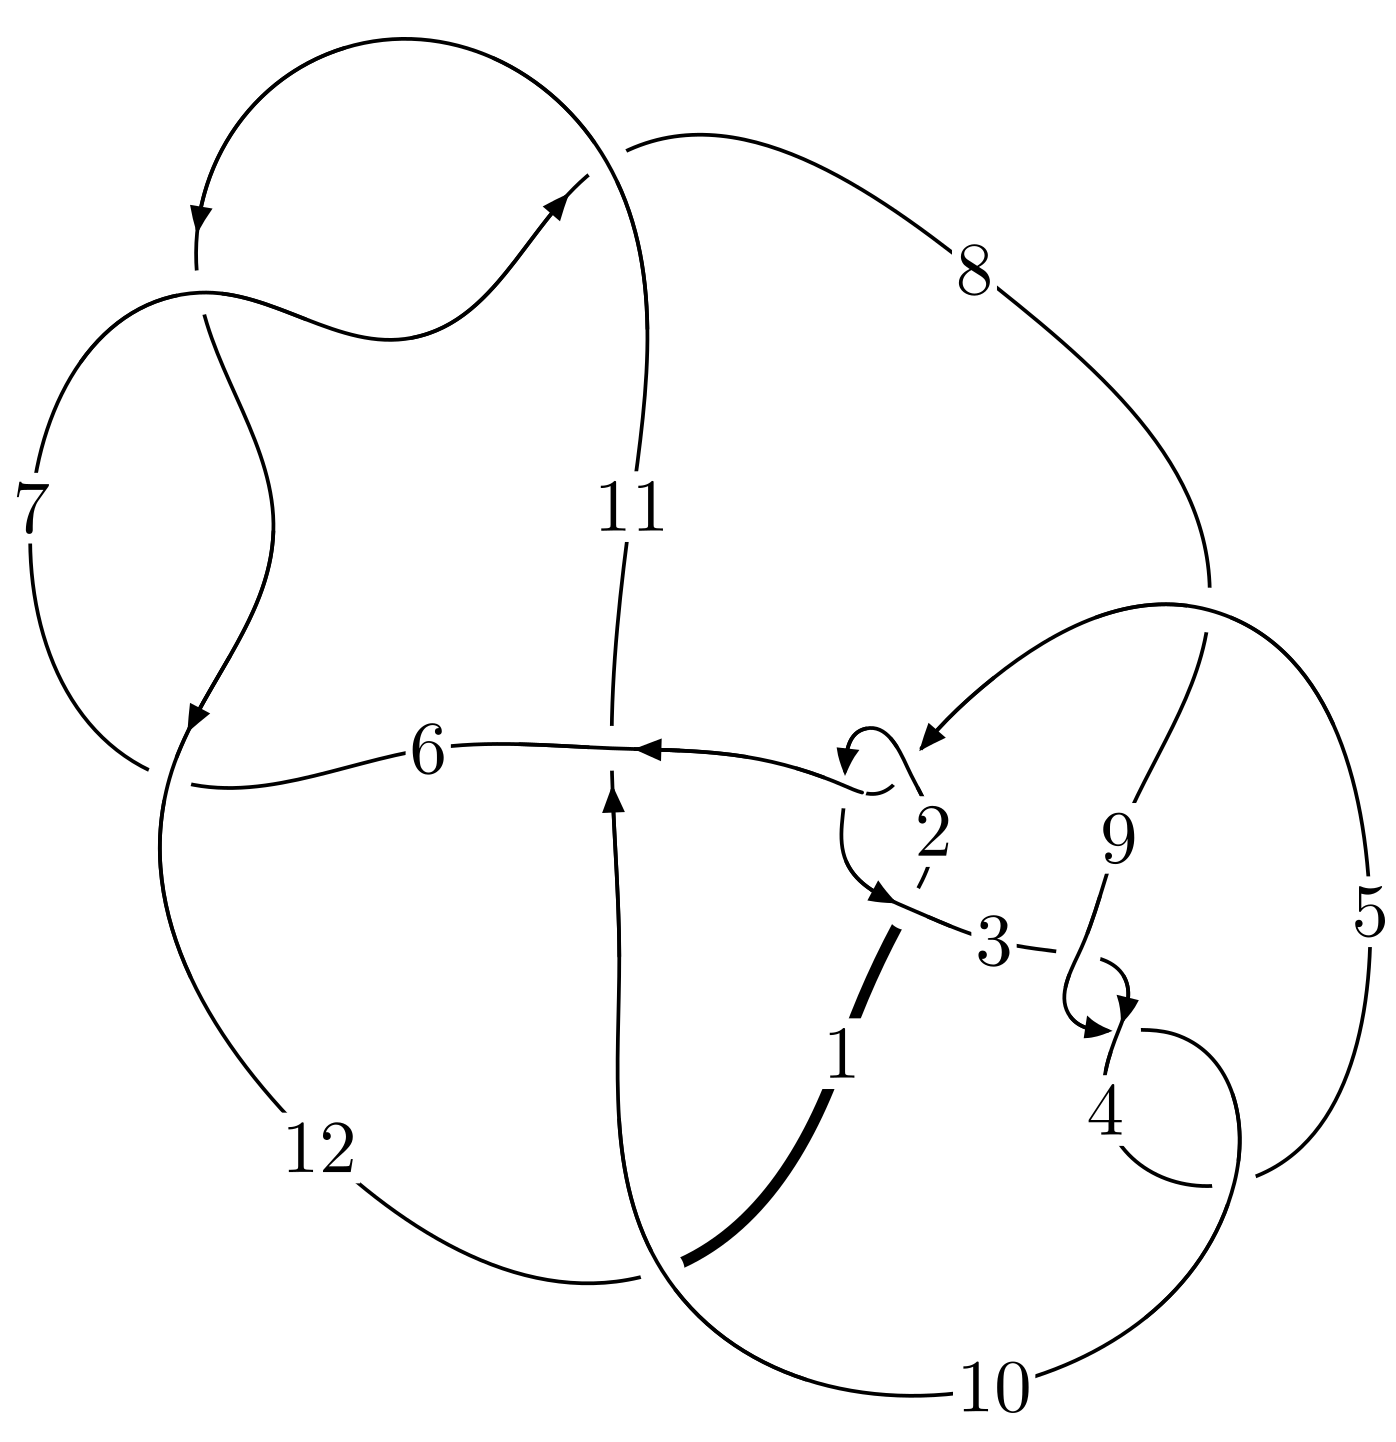
\includegraphics[width=112pt]{../../../GIT/diagram.site/Diagrams/png/2560_12n_0471.png}\\
\ \ \ A knot diagram\footnotemark}&
\allowdisplaybreaks
\textbf{Linearized knot diagam} \\
\cline{2-2}
 &
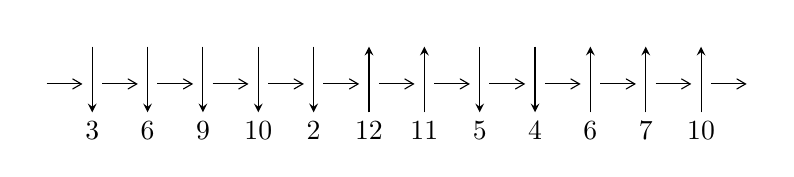
\begin{tikzpicture}[x=20pt, y=17pt]
	% nodes
	\node (C0) at (0, 0) {};
	\node (C1) at (1, 0) {};
	\node (C1U) at (1, +1) {};
	\node (C1D) at (1, -1) {3};

	\node (C2) at (2, 0) {};
	\node (C2U) at (2, +1) {};
	\node (C2D) at (2, -1) {6};

	\node (C3) at (3, 0) {};
	\node (C3U) at (3, +1) {};
	\node (C3D) at (3, -1) {9};

	\node (C4) at (4, 0) {};
	\node (C4U) at (4, +1) {};
	\node (C4D) at (4, -1) {10};

	\node (C5) at (5, 0) {};
	\node (C5U) at (5, +1) {};
	\node (C5D) at (5, -1) {2};

	\node (C6) at (6, 0) {};
	\node (C6U) at (6, +1) {};
	\node (C6D) at (6, -1) {12};

	\node (C7) at (7, 0) {};
	\node (C7U) at (7, +1) {};
	\node (C7D) at (7, -1) {11};

	\node (C8) at (8, 0) {};
	\node (C8U) at (8, +1) {};
	\node (C8D) at (8, -1) {5};

	\node (C9) at (9, 0) {};
	\node (C9U) at (9, +1) {};
	\node (C9D) at (9, -1) {4};

	\node (C10) at (10, 0) {};
	\node (C10U) at (10, +1) {};
	\node (C10D) at (10, -1) {6};

	\node (C11) at (11, 0) {};
	\node (C11U) at (11, +1) {};
	\node (C11D) at (11, -1) {7};

	\node (C12) at (12, 0) {};
	\node (C12U) at (12, +1) {};
	\node (C12D) at (12, -1) {10};
	\node (C13) at (13, 0) {};

	% arrows
	\draw[->,>={angle 60}]
	(C0) edge (C1) (C1) edge (C2) (C2) edge (C3) (C3) edge (C4) (C4) edge (C5) (C5) edge (C6) (C6) edge (C7) (C7) edge (C8) (C8) edge (C9) (C9) edge (C10) (C10) edge (C11) (C11) edge (C12) (C12) edge (C13) ;	\draw[->,>=stealth]
	(C1U) edge (C1D) (C2U) edge (C2D) (C3U) edge (C3D) (C4U) edge (C4D) (C5U) edge (C5D) (C6D) edge (C6U) (C7D) edge (C7U) (C8U) edge (C8D) (C9U) edge (C9D) (C10D) edge (C10U) (C11D) edge (C11U) (C12D) edge (C12U) ;
	\end{tikzpicture} \\
\hhline{~~} \\& 
\textbf{Solving Sequence} \\ \cline{2-2} 
 &
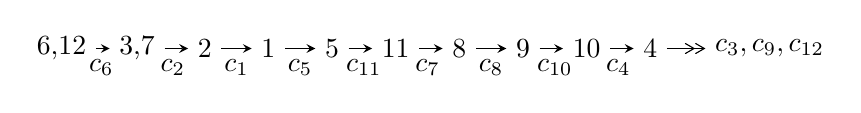
\begin{tikzpicture}[x=23pt, y=7pt]
	% node
	\node (A0) at (-1/8, 0) {6,12};
	\node (A1) at (17/16, 0) {3,7};
	\node (A2) at (17/8, 0) {2};
	\node (A3) at (25/8, 0) {1};
	\node (A4) at (33/8, 0) {5};
	\node (A5) at (41/8, 0) {11};
	\node (A6) at (49/8, 0) {8};
	\node (A7) at (57/8, 0) {9};
	\node (A8) at (65/8, 0) {10};
	\node (A9) at (73/8, 0) {4};
	\node (C1) at (1/2, -1) {$c_{6}$};
	\node (C2) at (13/8, -1) {$c_{2}$};
	\node (C3) at (21/8, -1) {$c_{1}$};
	\node (C4) at (29/8, -1) {$c_{5}$};
	\node (C5) at (37/8, -1) {$c_{11}$};
	\node (C6) at (45/8, -1) {$c_{7}$};
	\node (C7) at (53/8, -1) {$c_{8}$};
	\node (C8) at (61/8, -1) {$c_{10}$};
	\node (C9) at (69/8, -1) {$c_{4}$};
	\node (A10) at (11, 0) {$c_{3},c_{9},c_{12}$};

	% edge
	\draw[->,>=stealth]	
	(A0) edge (A1) (A1) edge (A2) (A2) edge (A3) (A3) edge (A4) (A4) edge (A5) (A5) edge (A6) (A6) edge (A7) (A7) edge (A8) (A8) edge (A9) ;
	\draw[->>,>={angle 60}]	
	(A9) edge (A10);
\end{tikzpicture} \\ 

\end{tabular} \\

\footnotetext{
The image of knot diagram is generated by the software ``\textbf{Draw programme}" developed by Andrew Bartholomew(\url{http://www.layer8.co.uk/maths/draw/index.htm\#Running-draw}), where we modified some parts for our purpose(\url{https://github.com/CATsTAILs/LinksPainter}).
}\phantom \\ \newline 
\centering \textbf{Ideals for irreducible components\footnotemark of $X_{\text{par}}$} 
 
\begin{align*}
I^u_{1}&=\langle 
-147633099219 u^{43}+379863908626 u^{42}+\cdots+592898388701 b-1077740574717,\\
\phantom{I^u_{1}}&\phantom{= \langle  }1873032055350 u^{43}-3613432711737 u^{42}+\cdots+1185796777402 a-16189929128661,\\
\phantom{I^u_{1}}&\phantom{= \langle  }u^{44}-2 u^{43}+\cdots-12 u-1\rangle \\
I^u_{2}&=\langle 
b-1,\;2 u^2 a+a^2-2 a u+4 a+u-1,\;u^3- u^2+2 u-1\rangle \\
I^u_{3}&=\langle 
b+1,\;- u^2+a- u-2,\;u^3+u^2+2 u+1\rangle \\
\\
\end{align*}
\raggedright * 3 irreducible components of $\dim_{\mathbb{C}}=0$, with total 53 representations.\\
\footnotetext{All coefficients of polynomials are rational numbers. But the coefficients are sometimes approximated in decimal forms when there is not enough margin.}
\newpage
\renewcommand{\arraystretch}{1}
\centering \section*{I. $I^u_{1}= \langle -1.48\times10^{11} u^{43}+3.80\times10^{11} u^{42}+\cdots+5.93\times10^{11} b-1.08\times10^{12},\;1.87\times10^{12} u^{43}-3.61\times10^{12} u^{42}+\cdots+1.19\times10^{12} a-1.62\times10^{13},\;u^{44}-2 u^{43}+\cdots-12 u-1 \rangle$}
\flushleft \textbf{(i) Arc colorings}\\
\begin{tabular}{m{7pt} m{180pt} m{7pt} m{180pt} }
\flushright $a_{6}=$&$\begin{pmatrix}1\\0\end{pmatrix}$ \\
\flushright $a_{12}=$&$\begin{pmatrix}0\\u\end{pmatrix}$ \\
\flushright $a_{3}=$&$\begin{pmatrix}-1.57956 u^{43}+3.04726 u^{42}+\cdots+15.8478 u+13.6532\\0.249002 u^{43}-0.640690 u^{42}+\cdots+7.19437 u+1.81775\end{pmatrix}$ \\
\flushright $a_{7}=$&$\begin{pmatrix}1\\- u^2\end{pmatrix}$ \\
\flushright $a_{2}=$&$\begin{pmatrix}-1.33055 u^{43}+2.40657 u^{42}+\cdots+23.0422 u+15.4710\\0.249002 u^{43}-0.640690 u^{42}+\cdots+7.19437 u+1.81775\end{pmatrix}$ \\
\flushright $a_{1}=$&$\begin{pmatrix}u^7+4 u^5+4 u^3\\- u^7-3 u^5-2 u^3+u\end{pmatrix}$ \\
\flushright $a_{5}=$&$\begin{pmatrix}1.94605 u^{43}-3.56049 u^{42}+\cdots-33.9928 u-16.2437\\-0.106829 u^{43}+0.292551 u^{42}+\cdots-3.38360 u-1.39701\end{pmatrix}$ \\
\flushright $a_{11}=$&$\begin{pmatrix}- u\\u^3+u\end{pmatrix}$ \\
\flushright $a_{8}=$&$\begin{pmatrix}u^2+1\\- u^4-2 u^2\end{pmatrix}$ \\
\flushright $a_{9}=$&$\begin{pmatrix}-1.90349 u^{43}+4.58255 u^{42}+\cdots+32.9049 u+21.3530\\-0.231468 u^{43}+0.479188 u^{42}+\cdots+1.51379 u+1.68525\end{pmatrix}$ \\
\flushright $a_{10}=$&$\begin{pmatrix}- u^3-2 u\\u^3+u\end{pmatrix}$ \\
\flushright $a_{4}=$&$\begin{pmatrix}1.63753 u^{43}-3.01547 u^{42}+\cdots-38.8903 u-16.9586\\0.0851016 u^{43}-0.122356 u^{42}+\cdots-0.258282 u-0.988042\end{pmatrix}$\\&\end{tabular}
\flushleft \textbf{(ii) Obstruction class $= -1$}\\~\\
\flushleft \textbf{(iii) Cusp Shapes $= -\frac{248546356620}{592898388701} u^{43}+\frac{1117851140785}{592898388701} u^{42}+\cdots-\frac{3366360188518}{592898388701} u-\frac{8799598819910}{592898388701}$}\\~\\
\newpage\renewcommand{\arraystretch}{1}
\flushleft \textbf{(iv) u-Polynomials at the component}\newline \\
\begin{tabular}{m{50pt}|m{274pt}}
Crossings & \hspace{64pt}u-Polynomials at each crossing \\
\hline $$\begin{aligned}c_{1}\end{aligned}$$&$\begin{aligned}
&u^{44}+14 u^{43}+\cdots+687 u+49
\end{aligned}$\\
\hline $$\begin{aligned}c_{2},c_{5}\end{aligned}$$&$\begin{aligned}
&u^{44}+4 u^{43}+\cdots+13 u-7
\end{aligned}$\\
\hline $$\begin{aligned}c_{3},c_{4},c_{9}\end{aligned}$$&$\begin{aligned}
&u^{44}- u^{43}+\cdots-8 u-8
\end{aligned}$\\
\hline $$\begin{aligned}c_{6},c_{7},c_{11}\end{aligned}$$&$\begin{aligned}
&u^{44}-2 u^{43}+\cdots-12 u-1
\end{aligned}$\\
\hline $$\begin{aligned}c_{8}\end{aligned}$$&$\begin{aligned}
&u^{44}+3 u^{43}+\cdots+8 u+8
\end{aligned}$\\
\hline $$\begin{aligned}c_{10}\end{aligned}$$&$\begin{aligned}
&u^{44}+2 u^{43}+\cdots-216 u-13
\end{aligned}$\\
\hline $$\begin{aligned}c_{12}\end{aligned}$$&$\begin{aligned}
&u^{44}+20 u^{43}+\cdots-582288 u+12161
\end{aligned}$\\
\hline
\end{tabular}\\~\\
\newpage\renewcommand{\arraystretch}{1}
\flushleft \textbf{(v) Riley Polynomials at the component}\newline \\
\begin{tabular}{m{50pt}|m{274pt}}
Crossings & \hspace{64pt}Riley Polynomials at each crossing \\
\hline $$\begin{aligned}c_{1}\end{aligned}$$&$\begin{aligned}
&y^{44}+42 y^{43}+\cdots-11859 y+2401
\end{aligned}$\\
\hline $$\begin{aligned}c_{2},c_{5}\end{aligned}$$&$\begin{aligned}
&y^{44}-14 y^{43}+\cdots-687 y+49
\end{aligned}$\\
\hline $$\begin{aligned}c_{3},c_{4},c_{9}\end{aligned}$$&$\begin{aligned}
&y^{44}-37 y^{43}+\cdots-64 y+64
\end{aligned}$\\
\hline $$\begin{aligned}c_{6},c_{7},c_{11}\end{aligned}$$&$\begin{aligned}
&y^{44}+36 y^{43}+\cdots-120 y+1
\end{aligned}$\\
\hline $$\begin{aligned}c_{8}\end{aligned}$$&$\begin{aligned}
&y^{44}+47 y^{43}+\cdots-960 y+64
\end{aligned}$\\
\hline $$\begin{aligned}c_{10}\end{aligned}$$&$\begin{aligned}
&y^{44}-44 y^{43}+\cdots-21852 y+169
\end{aligned}$\\
\hline $$\begin{aligned}c_{12}\end{aligned}$$&$\begin{aligned}
&y^{44}-68 y^{43}+\cdots-423863999800 y+147889921
\end{aligned}$\\
\hline
\end{tabular}\\~\\
\newpage\flushleft \textbf{(vi) Complex Volumes and Cusp Shapes}
$$\begin{array}{c|c|c}  
\text{Solutions to }I^u_{1}& \I (\text{vol} + \sqrt{-1}CS) & \text{Cusp shape}\\
 \hline 
\begin{aligned}
u &= \phantom{-}0.177625 + 1.046220 I \\
a &= \phantom{-}0.142421 - 1.282600 I \\
b &= -0.111509 + 0.704372 I\end{aligned}
 & -1.13792 + 1.81248 I & -1.86603 - 4.45266 I \\ \hline\begin{aligned}
u &= \phantom{-}0.177625 - 1.046220 I \\
a &= \phantom{-}0.142421 + 1.282600 I \\
b &= -0.111509 - 0.704372 I\end{aligned}
 & -1.13792 - 1.81248 I & -1.86603 + 4.45266 I \\ \hline\begin{aligned}
u &= -0.905481 + 0.047868 I \\
a &= -1.61810 - 2.71471 I \\
b &= \phantom{-}0.969501 + 0.973014 I\end{aligned}
 & \phantom{-}8.90320 - 3.55413 I & \phantom{-}1.57190 + 2.73369 I \\ \hline\begin{aligned}
u &= -0.905481 - 0.047868 I \\
a &= -1.61810 + 2.71471 I \\
b &= \phantom{-}0.969501 - 0.973014 I\end{aligned}
 & \phantom{-}8.90320 + 3.55413 I & \phantom{-}1.57190 - 2.73369 I \\ \hline\begin{aligned}
u &= \phantom{-}0.888633 + 0.113112 I \\
a &= \phantom{-}1.63253 - 2.72104 I \\
b &= -1.13181 + 0.84989 I\end{aligned}
 & \phantom{-}4.21307 + 8.73460 I & -2.10151 - 5.42806 I \\ \hline\begin{aligned}
u &= \phantom{-}0.888633 - 0.113112 I \\
a &= \phantom{-}1.63253 + 2.72104 I \\
b &= -1.13181 - 0.84989 I\end{aligned}
 & \phantom{-}4.21307 - 8.73460 I & -2.10151 + 5.42806 I \\ \hline\begin{aligned}
u &= \phantom{-}0.895146 + 0.030335 I \\
a &= \phantom{-}1.50372 + 2.63941 I \\
b &= -0.725758 - 1.037770 I\end{aligned}
 & \phantom{-}5.49591 + 1.83935 I & -0.526060 - 1.054264 I \\ \hline\begin{aligned}
u &= \phantom{-}0.895146 - 0.030335 I \\
a &= \phantom{-}1.50372 - 2.63941 I \\
b &= -0.725758 + 1.037770 I\end{aligned}
 & \phantom{-}5.49591 - 1.83935 I & -0.526060 + 1.054264 I \\ \hline\begin{aligned}
u &= -0.124146 + 1.195890 I \\
a &= \phantom{-}0.103513 + 1.322400 I \\
b &= -1.136390 - 0.239685 I\end{aligned}
 & -4.44373 - 1.62575 I & -5.71135 - 1.58189 I \\ \hline\begin{aligned}
u &= -0.124146 - 1.195890 I \\
a &= \phantom{-}0.103513 - 1.322400 I \\
b &= -1.136390 + 0.239685 I\end{aligned}
 & -4.44373 + 1.62575 I & -5.71135 + 1.58189 I\\
 \hline 
 \end{array}$$\newpage$$\begin{array}{c|c|c}  
\text{Solutions to }I^u_{1}& \I (\text{vol} + \sqrt{-1}CS) & \text{Cusp shape}\\
 \hline 
\begin{aligned}
u &= -0.028993 + 1.237360 I \\
a &= \phantom{-}0.27041 + 1.84256 I \\
b &= \phantom{-}1.116190 - 0.284540 I\end{aligned}
 & -10.24070 - 0.43963 I & -11.19118 - 0.81443 I \\ \hline\begin{aligned}
u &= -0.028993 - 1.237360 I \\
a &= \phantom{-}0.27041 - 1.84256 I \\
b &= \phantom{-}1.116190 + 0.284540 I\end{aligned}
 & -10.24070 + 0.43963 I & -11.19118 + 0.81443 I \\ \hline\begin{aligned}
u &= \phantom{-}0.755269\phantom{ +0.000000I} \\
a &= -2.04829\phantom{ +0.000000I} \\
b &= \phantom{-}1.32092\phantom{ +0.000000I}\end{aligned}
 & -2.54326\phantom{ +0.000000I} & -3.28070\phantom{ +0.000000I} \\ \hline\begin{aligned}
u &= \phantom{-}0.453023 + 1.165750 I \\
a &= \phantom{-}1.46711 + 1.23873 I \\
b &= -1.053650 - 0.886079 I\end{aligned}
 & \phantom{-}0.98373 - 3.94476 I & -4.68762 + 2.02851 I \\ \hline\begin{aligned}
u &= \phantom{-}0.453023 - 1.165750 I \\
a &= \phantom{-}1.46711 - 1.23873 I \\
b &= -1.053650 + 0.886079 I\end{aligned}
 & \phantom{-}0.98373 + 3.94476 I & -4.68762 - 2.02851 I \\ \hline\begin{aligned}
u &= -0.254381 + 1.244050 I \\
a &= -1.35227 - 1.46538 I \\
b &= \phantom{-}0.461470 + 0.356687 I\end{aligned}
 & -7.86357 - 3.29517 I & -5.01423 + 4.50472 I \\ \hline\begin{aligned}
u &= -0.254381 - 1.244050 I \\
a &= -1.35227 + 1.46538 I \\
b &= \phantom{-}0.461470 - 0.356687 I\end{aligned}
 & -7.86357 + 3.29517 I & -5.01423 - 4.50472 I \\ \hline\begin{aligned}
u &= -0.530116 + 0.484400 I \\
a &= \phantom{-}0.22811 + 1.92477 I \\
b &= -0.793793 - 0.687491 I\end{aligned}
 & -1.89298 - 4.16205 I & -4.34545 + 6.93236 I \\ \hline\begin{aligned}
u &= -0.530116 - 0.484400 I \\
a &= \phantom{-}0.22811 - 1.92477 I \\
b &= -0.793793 + 0.687491 I\end{aligned}
 & -1.89298 + 4.16205 I & -4.34545 - 6.93236 I \\ \hline\begin{aligned}
u &= \phantom{-}0.319810 + 1.254700 I \\
a &= -0.613086 + 0.914327 I \\
b &= \phantom{-}1.341730 + 0.022586 I\end{aligned}
 & -6.42106 + 3.87791 I & -7.73542 - 3.96367 I\\
 \hline 
 \end{array}$$\newpage$$\begin{array}{c|c|c}  
\text{Solutions to }I^u_{1}& \I (\text{vol} + \sqrt{-1}CS) & \text{Cusp shape}\\
 \hline 
\begin{aligned}
u &= \phantom{-}0.319810 - 1.254700 I \\
a &= -0.613086 - 0.914327 I \\
b &= \phantom{-}1.341730 - 0.022586 I\end{aligned}
 & -6.42106 - 3.87791 I & -7.73542 + 3.96367 I \\ \hline\begin{aligned}
u &= -0.447807 + 1.241790 I \\
a &= -1.49241 + 1.30249 I \\
b &= \phantom{-}0.865876 - 1.008920 I\end{aligned}
 & \phantom{-}5.21565 - 1.27455 I & \phantom{-0.000000 } 0 \\ \hline\begin{aligned}
u &= -0.447807 - 1.241790 I \\
a &= -1.49241 - 1.30249 I \\
b &= \phantom{-}0.865876 + 1.008920 I\end{aligned}
 & \phantom{-}5.21565 + 1.27455 I & \phantom{-0.000000 } 0 \\ \hline\begin{aligned}
u &= \phantom{-}0.431847 + 1.254620 I \\
a &= \phantom{-}0.25969 - 2.31831 I \\
b &= -0.822510 + 0.981509 I\end{aligned}
 & \phantom{-}1.70650 + 2.90262 I & \phantom{-0.000000 } 0 \\ \hline\begin{aligned}
u &= \phantom{-}0.431847 - 1.254620 I \\
a &= \phantom{-}0.25969 + 2.31831 I \\
b &= -0.822510 - 0.981509 I\end{aligned}
 & \phantom{-}1.70650 - 2.90262 I & \phantom{-0.000000 } 0 \\ \hline\begin{aligned}
u &= -0.657910\phantom{ +0.000000I} \\
a &= -2.47446\phantom{ +0.000000I} \\
b &= \phantom{-}0.397664\phantom{ +0.000000I}\end{aligned}
 & -4.04738\phantom{ +0.000000I} & \phantom{-}1.08600\phantom{ +0.000000I} \\ \hline\begin{aligned}
u &= -0.509311 + 0.393833 I \\
a &= \phantom{-}1.131640 - 0.668056 I \\
b &= -0.669143 + 0.583071 I\end{aligned}
 & -1.77451 + 0.52923 I & -4.16249 + 0.21334 I \\ \hline\begin{aligned}
u &= -0.509311 - 0.393833 I \\
a &= \phantom{-}1.131640 + 0.668056 I \\
b &= -0.669143 - 0.583071 I\end{aligned}
 & -1.77451 - 0.52923 I & -4.16249 - 0.21334 I \\ \hline\begin{aligned}
u &= \phantom{-}0.420827 + 1.304130 I \\
a &= \phantom{-}1.42832 + 1.31723 I \\
b &= -0.626328 - 1.065560 I\end{aligned}
 & \phantom{-}1.33689 + 6.54913 I & \phantom{-0.000000 } 0 \\ \hline\begin{aligned}
u &= \phantom{-}0.420827 - 1.304130 I \\
a &= \phantom{-}1.42832 - 1.31723 I \\
b &= -0.626328 + 1.065560 I\end{aligned}
 & \phantom{-}1.33689 - 6.54913 I & \phantom{-0.000000 } 0\\
 \hline 
 \end{array}$$\newpage$$\begin{array}{c|c|c}  
\text{Solutions to }I^u_{1}& \I (\text{vol} + \sqrt{-1}CS) & \text{Cusp shape}\\
 \hline 
\begin{aligned}
u &= \phantom{-}0.181384 + 1.359970 I \\
a &= \phantom{-}0.407588 + 0.745307 I \\
b &= \phantom{-}0.699749 - 0.288589 I\end{aligned}
 & -4.01419 + 3.49485 I & \phantom{-0.000000 } 0 \\ \hline\begin{aligned}
u &= \phantom{-}0.181384 - 1.359970 I \\
a &= \phantom{-}0.407588 - 0.745307 I \\
b &= \phantom{-}0.699749 + 0.288589 I\end{aligned}
 & -4.01419 - 3.49485 I & \phantom{-0.000000 } 0 \\ \hline\begin{aligned}
u &= -0.423050 + 1.318510 I \\
a &= -0.24113 - 2.42704 I \\
b &= \phantom{-}1.046820 + 0.917522 I\end{aligned}
 & \phantom{-}4.63663 - 8.30735 I & \phantom{-0.000000 } 0 \\ \hline\begin{aligned}
u &= -0.423050 - 1.318510 I \\
a &= -0.24113 + 2.42704 I \\
b &= \phantom{-}1.046820 - 0.917522 I\end{aligned}
 & \phantom{-}4.63663 + 8.30735 I & \phantom{-0.000000 } 0 \\ \hline\begin{aligned}
u &= -0.192973 + 1.390020 I \\
a &= \phantom{-}0.1114790 + 0.0226378 I \\
b &= -0.666441 + 0.485044 I\end{aligned}
 & -7.33799 - 1.99899 I & \phantom{-0.000000 } 0 \\ \hline\begin{aligned}
u &= -0.192973 - 1.390020 I \\
a &= \phantom{-}0.1114790 - 0.0226378 I \\
b &= -0.666441 - 0.485044 I\end{aligned}
 & -7.33799 + 1.99899 I & \phantom{-0.000000 } 0 \\ \hline\begin{aligned}
u &= \phantom{-}0.397923 + 1.355450 I \\
a &= \phantom{-}0.17147 - 2.46591 I \\
b &= -1.17690 + 0.80462 I\end{aligned}
 & -0.40257 + 13.35110 I & \phantom{-0.000000 } 0 \\ \hline\begin{aligned}
u &= \phantom{-}0.397923 - 1.355450 I \\
a &= \phantom{-}0.17147 + 2.46591 I \\
b &= -1.17690 - 0.80462 I\end{aligned}
 & -0.40257 - 13.35110 I & \phantom{-0.000000 } 0 \\ \hline\begin{aligned}
u &= \phantom{-}0.536600 + 0.237972 I \\
a &= \phantom{-}0.147433 + 1.338600 I \\
b &= \phantom{-}0.375946 - 0.435344 I\end{aligned}
 & \phantom{-}1.05918 + 0.97127 I & \phantom{-}3.52880 - 3.41320 I \\ \hline\begin{aligned}
u &= \phantom{-}0.536600 - 0.237972 I \\
a &= \phantom{-}0.147433 - 1.338600 I \\
b &= \phantom{-}0.375946 + 0.435344 I\end{aligned}
 & \phantom{-}1.05918 - 0.97127 I & \phantom{-}3.52880 + 3.41320 I\\
 \hline 
 \end{array}$$\newpage$$\begin{array}{c|c|c}  
\text{Solutions to }I^u_{1}& \I (\text{vol} + \sqrt{-1}CS) & \text{Cusp shape}\\
 \hline 
\begin{aligned}
u &= -0.13547 + 1.42408 I \\
a &= -0.481300 + 0.967134 I \\
b &= -0.921093 - 0.597509 I\end{aligned}
 & -8.04171 - 6.36604 I & \phantom{-0.000000 } 0 \\ \hline\begin{aligned}
u &= -0.13547 - 1.42408 I \\
a &= -0.481300 - 0.967134 I \\
b &= -0.921093 + 0.597509 I\end{aligned}
 & -8.04171 + 6.36604 I & \phantom{-0.000000 } 0 \\ \hline\begin{aligned}
u &= -0.302868\phantom{ +0.000000I} \\
a &= \phantom{-}2.56595\phantom{ +0.000000I} \\
b &= -0.846938\phantom{ +0.000000I}\end{aligned}
 & -1.10522\phantom{ +0.000000I} & -12.4510\phantom{ +0.000000I} \\ \hline\begin{aligned}
u &= -0.0966649\phantom{ +0.000000I} \\
a &= \phantom{-}11.5425\phantom{ +0.000000I} \\
b &= \phantom{-}1.04441\phantom{ +0.000000I}\end{aligned}
 & -6.54665\phantom{ +0.000000I} & -14.0770\phantom{ +0.000000I}\\
 \hline 
 \end{array}$$\newpage\newpage\renewcommand{\arraystretch}{1}
\centering \section*{II. $I^u_{2}= \langle b-1,\;2 u^2 a+a^2-2 a u+4 a+u-1,\;u^3- u^2+2 u-1 \rangle$}
\flushleft \textbf{(i) Arc colorings}\\
\begin{tabular}{m{7pt} m{180pt} m{7pt} m{180pt} }
\flushright $a_{6}=$&$\begin{pmatrix}1\\0\end{pmatrix}$ \\
\flushright $a_{12}=$&$\begin{pmatrix}0\\u\end{pmatrix}$ \\
\flushright $a_{3}=$&$\begin{pmatrix}a\\1\end{pmatrix}$ \\
\flushright $a_{7}=$&$\begin{pmatrix}1\\- u^2\end{pmatrix}$ \\
\flushright $a_{2}=$&$\begin{pmatrix}a+1\\1\end{pmatrix}$ \\
\flushright $a_{1}=$&$\begin{pmatrix}1\\0\end{pmatrix}$ \\
\flushright $a_{5}=$&$\begin{pmatrix}- a\\-1\end{pmatrix}$ \\
\flushright $a_{11}=$&$\begin{pmatrix}- u\\u^2- u+1\end{pmatrix}$ \\
\flushright $a_{8}=$&$\begin{pmatrix}u^2+1\\- u^2+u-1\end{pmatrix}$ \\
\flushright $a_{9}=$&$\begin{pmatrix}- u^2 a+2 u^2- a+1\\u^2 a- a u+a+u\end{pmatrix}$ \\
\flushright $a_{10}=$&$\begin{pmatrix}- u^2-1\\u^2- u+1\end{pmatrix}$ \\
\flushright $a_{4}=$&$\begin{pmatrix}- u^2-2 a+u-2\\a u\end{pmatrix}$\\&\end{tabular}
\flushleft \textbf{(ii) Obstruction class $= 1$}\\~\\
\flushleft \textbf{(iii) Cusp Shapes $= 4 u^2-4 u-4$}\\~\\
\newpage\renewcommand{\arraystretch}{1}
\flushleft \textbf{(iv) u-Polynomials at the component}\newline \\
\begin{tabular}{m{50pt}|m{274pt}}
Crossings & \hspace{64pt}u-Polynomials at each crossing \\
\hline $$\begin{aligned}c_{1},c_{5}\end{aligned}$$&$\begin{aligned}
&(u-1)^6
\end{aligned}$\\
\hline $$\begin{aligned}c_{2}\end{aligned}$$&$\begin{aligned}
&(u+1)^6
\end{aligned}$\\
\hline $$\begin{aligned}c_{3},c_{4},c_{8}\\c_{9}\end{aligned}$$&$\begin{aligned}
&(u^2-2)^3
\end{aligned}$\\
\hline $$\begin{aligned}c_{6},c_{7}\end{aligned}$$&$\begin{aligned}
&(u^3- u^2+2 u-1)^2
\end{aligned}$\\
\hline $$\begin{aligned}c_{10}\end{aligned}$$&$\begin{aligned}
&(u^3- u^2+1)^2
\end{aligned}$\\
\hline $$\begin{aligned}c_{11}\end{aligned}$$&$\begin{aligned}
&(u^3+u^2+2 u+1)^2
\end{aligned}$\\
\hline $$\begin{aligned}c_{12}\end{aligned}$$&$\begin{aligned}
&(u^3+u^2-1)^2
\end{aligned}$\\
\hline
\end{tabular}\\~\\
\newpage\renewcommand{\arraystretch}{1}
\flushleft \textbf{(v) Riley Polynomials at the component}\newline \\
\begin{tabular}{m{50pt}|m{274pt}}
Crossings & \hspace{64pt}Riley Polynomials at each crossing \\
\hline $$\begin{aligned}c_{1},c_{2},c_{5}\end{aligned}$$&$\begin{aligned}
&(y-1)^6
\end{aligned}$\\
\hline $$\begin{aligned}c_{3},c_{4},c_{8}\\c_{9}\end{aligned}$$&$\begin{aligned}
&(y-2)^6
\end{aligned}$\\
\hline $$\begin{aligned}c_{6},c_{7},c_{11}\end{aligned}$$&$\begin{aligned}
&(y^3+3 y^2+2 y-1)^2
\end{aligned}$\\
\hline $$\begin{aligned}c_{10},c_{12}\end{aligned}$$&$\begin{aligned}
&(y^3- y^2+2 y-1)^2
\end{aligned}$\\
\hline
\end{tabular}\\~\\
\newpage\flushleft \textbf{(vi) Complex Volumes and Cusp Shapes}
$$\begin{array}{c|c|c}  
\text{Solutions to }I^u_{2}& \I (\text{vol} + \sqrt{-1}CS) & \text{Cusp shape}\\
 \hline 
\begin{aligned}
u &= \phantom{-}0.215080 + 1.307140 I \\
a &= \phantom{-}0.814156 - 0.050322 I \\
b &= \phantom{-}1.00000\phantom{ +0.000000I}\end{aligned}
 & -9.60386 + 2.82812 I & -11.50976 - 2.97945 I \\ \hline\begin{aligned}
u &= \phantom{-}0.215080 + 1.307140 I \\
a &= -1.05928 + 1.54005 I \\
b &= \phantom{-}1.00000\phantom{ +0.000000I}\end{aligned}
 & -9.60386 + 2.82812 I & -11.50976 - 2.97945 I \\ \hline\begin{aligned}
u &= \phantom{-}0.215080 - 1.307140 I \\
a &= \phantom{-}0.814156 + 0.050322 I \\
b &= \phantom{-}1.00000\phantom{ +0.000000I}\end{aligned}
 & -9.60386 - 2.82812 I & -11.50976 + 2.97945 I \\ \hline\begin{aligned}
u &= \phantom{-}0.215080 - 1.307140 I \\
a &= -1.05928 - 1.54005 I \\
b &= \phantom{-}1.00000\phantom{ +0.000000I}\end{aligned}
 & -9.60386 - 2.82812 I & -11.50976 + 2.97945 I \\ \hline\begin{aligned}
u &= \phantom{-}0.569840\phantom{ +0.000000I} \\
a &= \phantom{-}0.118556\phantom{ +0.000000I} \\
b &= \phantom{-}1.00000\phantom{ +0.000000I}\end{aligned}
 & -5.46628\phantom{ +0.000000I} & -4.98050\phantom{ +0.000000I} \\ \hline\begin{aligned}
u &= \phantom{-}0.569840\phantom{ +0.000000I} \\
a &= -3.62831\phantom{ +0.000000I} \\
b &= \phantom{-}1.00000\phantom{ +0.000000I}\end{aligned}
 & -5.46628\phantom{ +0.000000I} & -4.98050\phantom{ +0.000000I}\\
 \hline 
 \end{array}$$\newpage\newpage\renewcommand{\arraystretch}{1}
\centering \section*{III. $I^u_{3}= \langle b+1,\;- u^2+a- u-2,\;u^3+u^2+2 u+1 \rangle$}
\flushleft \textbf{(i) Arc colorings}\\
\begin{tabular}{m{7pt} m{180pt} m{7pt} m{180pt} }
\flushright $a_{6}=$&$\begin{pmatrix}1\\0\end{pmatrix}$ \\
\flushright $a_{12}=$&$\begin{pmatrix}0\\u\end{pmatrix}$ \\
\flushright $a_{3}=$&$\begin{pmatrix}u^2+u+2\\-1\end{pmatrix}$ \\
\flushright $a_{7}=$&$\begin{pmatrix}1\\- u^2\end{pmatrix}$ \\
\flushright $a_{2}=$&$\begin{pmatrix}u^2+u+1\\-1\end{pmatrix}$ \\
\flushright $a_{1}=$&$\begin{pmatrix}-1\\0\end{pmatrix}$ \\
\flushright $a_{5}=$&$\begin{pmatrix}u^2+u+2\\-1\end{pmatrix}$ \\
\flushright $a_{11}=$&$\begin{pmatrix}- u\\- u^2- u-1\end{pmatrix}$ \\
\flushright $a_{8}=$&$\begin{pmatrix}u^2+1\\- u^2- u-1\end{pmatrix}$ \\
\flushright $a_{9}=$&$\begin{pmatrix}u^2+1\\- u^2- u-1\end{pmatrix}$ \\
\flushright $a_{10}=$&$\begin{pmatrix}u^2+1\\- u^2- u-1\end{pmatrix}$ \\
\flushright $a_{4}=$&$\begin{pmatrix}u^2+u+2\\-1\end{pmatrix}$\\&\end{tabular}
\flushleft \textbf{(ii) Obstruction class $= 1$}\\~\\
\flushleft \textbf{(iii) Cusp Shapes $= 6 u^2+4 u+4$}\\~\\
\newpage\renewcommand{\arraystretch}{1}
\flushleft \textbf{(iv) u-Polynomials at the component}\newline \\
\begin{tabular}{m{50pt}|m{274pt}}
Crossings & \hspace{64pt}u-Polynomials at each crossing \\
\hline $$\begin{aligned}c_{1},c_{2}\end{aligned}$$&$\begin{aligned}
&(u-1)^3
\end{aligned}$\\
\hline $$\begin{aligned}c_{3},c_{4},c_{8}\\c_{9}\end{aligned}$$&$\begin{aligned}
&u^3
\end{aligned}$\\
\hline $$\begin{aligned}c_{5}\end{aligned}$$&$\begin{aligned}
&(u+1)^3
\end{aligned}$\\
\hline $$\begin{aligned}c_{6},c_{7}\end{aligned}$$&$\begin{aligned}
&u^3+u^2+2 u+1
\end{aligned}$\\
\hline $$\begin{aligned}c_{10},c_{12}\end{aligned}$$&$\begin{aligned}
&u^3+u^2-1
\end{aligned}$\\
\hline $$\begin{aligned}c_{11}\end{aligned}$$&$\begin{aligned}
&u^3- u^2+2 u-1
\end{aligned}$\\
\hline
\end{tabular}\\~\\
\newpage\renewcommand{\arraystretch}{1}
\flushleft \textbf{(v) Riley Polynomials at the component}\newline \\
\begin{tabular}{m{50pt}|m{274pt}}
Crossings & \hspace{64pt}Riley Polynomials at each crossing \\
\hline $$\begin{aligned}c_{1},c_{2},c_{5}\end{aligned}$$&$\begin{aligned}
&(y-1)^3
\end{aligned}$\\
\hline $$\begin{aligned}c_{3},c_{4},c_{8}\\c_{9}\end{aligned}$$&$\begin{aligned}
&y^3
\end{aligned}$\\
\hline $$\begin{aligned}c_{6},c_{7},c_{11}\end{aligned}$$&$\begin{aligned}
&y^3+3 y^2+2 y-1
\end{aligned}$\\
\hline $$\begin{aligned}c_{10},c_{12}\end{aligned}$$&$\begin{aligned}
&y^3- y^2+2 y-1
\end{aligned}$\\
\hline
\end{tabular}\\~\\
\newpage\flushleft \textbf{(vi) Complex Volumes and Cusp Shapes}
$$\begin{array}{c|c|c}  
\text{Solutions to }I^u_{3}& \I (\text{vol} + \sqrt{-1}CS) & \text{Cusp shape}\\
 \hline 
\begin{aligned}
u &= -0.215080 + 1.307140 I \\
a &= \phantom{-}0.122561 + 0.744862 I \\
b &= -1.00000\phantom{ +0.000000I}\end{aligned}
 & -4.66906 - 2.82812 I & -6.83447 + 1.85489 I \\ \hline\begin{aligned}
u &= -0.215080 - 1.307140 I \\
a &= \phantom{-}0.122561 - 0.744862 I \\
b &= -1.00000\phantom{ +0.000000I}\end{aligned}
 & -4.66906 + 2.82812 I & -6.83447 - 1.85489 I \\ \hline\begin{aligned}
u &= -0.569840\phantom{ +0.000000I} \\
a &= \phantom{-}1.75488\phantom{ +0.000000I} \\
b &= -1.00000\phantom{ +0.000000I}\end{aligned}
 & -0.531480\phantom{ +0.000000I} & \phantom{-}3.66890\phantom{ +0.000000I}\\
 \hline 
 \end{array}$$\newpage
\newpage\renewcommand{\arraystretch}{1}
\centering \section*{ IV. u-Polynomials}
\begin{tabular}{m{50pt}|m{274pt}}
Crossings & \hspace{64pt}u-Polynomials at each crossing \\
\hline $$\begin{aligned}c_{1}\end{aligned}$$&$\begin{aligned}
&((u-1)^9)(u^{44}+14 u^{43}+\cdots+687 u+49)
\end{aligned}$\\
\hline $$\begin{aligned}c_{2}\end{aligned}$$&$\begin{aligned}
&((u-1)^3)(u+1)^6(u^{44}+4 u^{43}+\cdots+13 u-7)
\end{aligned}$\\
\hline $$\begin{aligned}c_{3},c_{4},c_{9}\end{aligned}$$&$\begin{aligned}
&u^3(u^2-2)^3(u^{44}- u^{43}+\cdots-8 u-8)
\end{aligned}$\\
\hline $$\begin{aligned}c_{5}\end{aligned}$$&$\begin{aligned}
&((u-1)^6)(u+1)^3(u^{44}+4 u^{43}+\cdots+13 u-7)
\end{aligned}$\\
\hline $$\begin{aligned}c_{6},c_{7}\end{aligned}$$&$\begin{aligned}
&((u^3- u^2+2 u-1)^2)(u^3+u^2+2 u+1)(u^{44}-2 u^{43}+\cdots-12 u-1)
\end{aligned}$\\
\hline $$\begin{aligned}c_{8}\end{aligned}$$&$\begin{aligned}
&u^3(u^2-2)^3(u^{44}+3 u^{43}+\cdots+8 u+8)
\end{aligned}$\\
\hline $$\begin{aligned}c_{10}\end{aligned}$$&$\begin{aligned}
&((u^3- u^2+1)^2)(u^3+u^2-1)(u^{44}+2 u^{43}+\cdots-216 u-13)
\end{aligned}$\\
\hline $$\begin{aligned}c_{11}\end{aligned}$$&$\begin{aligned}
&(u^3- u^2+2 u-1)(u^3+u^2+2 u+1)^2(u^{44}-2 u^{43}+\cdots-12 u-1)
\end{aligned}$\\
\hline $$\begin{aligned}c_{12}\end{aligned}$$&$\begin{aligned}
&((u^3+u^2-1)^3)(u^{44}+20 u^{43}+\cdots-582288 u+12161)
\end{aligned}$\\
\hline
\end{tabular}\newpage\renewcommand{\arraystretch}{1}
\centering \section*{ V. Riley Polynomials}
\begin{tabular}{m{50pt}|m{274pt}}
Crossings & \hspace{64pt}Riley Polynomials at each crossing \\
\hline $$\begin{aligned}c_{1}\end{aligned}$$&$\begin{aligned}
&((y-1)^9)(y^{44}+42 y^{43}+\cdots-11859 y+2401)
\end{aligned}$\\
\hline $$\begin{aligned}c_{2},c_{5}\end{aligned}$$&$\begin{aligned}
&((y-1)^9)(y^{44}-14 y^{43}+\cdots-687 y+49)
\end{aligned}$\\
\hline $$\begin{aligned}c_{3},c_{4},c_{9}\end{aligned}$$&$\begin{aligned}
&y^3(y-2)^6(y^{44}-37 y^{43}+\cdots-64 y+64)
\end{aligned}$\\
\hline $$\begin{aligned}c_{6},c_{7},c_{11}\end{aligned}$$&$\begin{aligned}
&((y^3+3 y^2+2 y-1)^3)(y^{44}+36 y^{43}+\cdots-120 y+1)
\end{aligned}$\\
\hline $$\begin{aligned}c_{8}\end{aligned}$$&$\begin{aligned}
&y^3(y-2)^6(y^{44}+47 y^{43}+\cdots-960 y+64)
\end{aligned}$\\
\hline $$\begin{aligned}c_{10}\end{aligned}$$&$\begin{aligned}
&((y^3- y^2+2 y-1)^3)(y^{44}-44 y^{43}+\cdots-21852 y+169)
\end{aligned}$\\
\hline $$\begin{aligned}c_{12}\end{aligned}$$&$\begin{aligned}
&(y^3- y^2+2 y-1)^3\\
&\cdot(y^{44}-68 y^{43}+\cdots-423863999800 y+147889921)
\end{aligned}$\\
\hline
\end{tabular}
\vskip 2pc
\end{document}